




\chapter{Validation of Injection Channel}

Without loss of generality, We injected several binary blackhole (BBH) signals into PCal to test the performance of our De-Whitening Filter. Unfortunately, at this moment, we couldn't find a compatible data-taking system with desired noise level and dynamical range to faithfully reconstruct or estimate the expect End-Test Mirror (ETM) displacement that caused by our Photon Calibrator. The reason is that the ADC we used has much larger noise than the DAC we used. To beat the ADC noise, although we can amplify the signal before feeding it into the ADC, as what we did for noise measurement in last chapter, some part of injected waveform can easily saturate our ADC. Therefore, the results showed in this chapter should be treated as a demonstration of injecting simulated GW waveforms to PCal. The result should not be used for estimating noise performance.

In Fig.~\ref{fig:bbhinj}, we have chosen three different binary blackholes (BBH) coalescence waveform templates. All of them are equal-mass BBH system whose individual masses are 10, 20, and 30 solar mass correspondingly. They could have different portion of their signal that fit into the most sensitive frequency of the KAGRA detector. This can be helpful for some purposes, e.g.~testing General Relativity \cite{ligo:o1bbh}. If we can inject these signals into our main interferometer in the future, we could have a chance to test the response of KAGRA to these injections, thereby contributing to related BBH analysis works. The distance from the source to the detector is set to be 100 Mpc, which is a relative optimistic choice.

The injected waveform template is originally generated by \emph{IMRPhenomD}\footnote{IMRPhenomD is a phenomenological binary blackhole coalescence waveform generating method including both Inspiral, Merger, and Ringdown phase.} code in \emph{LALSuite}\footnote{LALSuite is the LIGO Scientific Collaboration Algorithm Library Suite.}. We selected a polarization mode of the strain waveform and translated it into the expected differential arm length change of 3 km KAGRA arms. Then, we calculated the required PCal power modulation according to Eq.~(\ref{eq:pcaldispt}). Next, the signal was injected through the \emph{multiawgstream}\footnote{multiawgstream is a program design by LIGO for injecting time series data into a specified channel in realtime models. In our case, the signal will be sent to PCal control model and result in corresponding DAC output for PCal laser intensity control. } program to the PCal control realtime model, in which the digital inverse De-Whitening filter has been implemented. Finally the output from Digital System was fed into our De-Whitening filter, and sent to the excitation port of our PCal, thereby modulating the intensity of PCal output laser beams. 

One thing I have to mention here is that when we perform the injection test, the absolute Laser Intensity of our PCal is not calibrated accurately yet. In the future we have to calibrate it by a customized power meter, i.e.~the Working Standard KAGRA (WSK), which is an integrating sphere followed by a photodiode and could be used for cross checking the absolute intensity of each PCal lasers across the worldwide gravitational wave detector network and also the laser power standard in some institutes, e.g.~NIST\footnote{NIST is the National Institute of Standards and Technology in the United States.}.
 


  

\begin{figure}[hbt!]
\centering
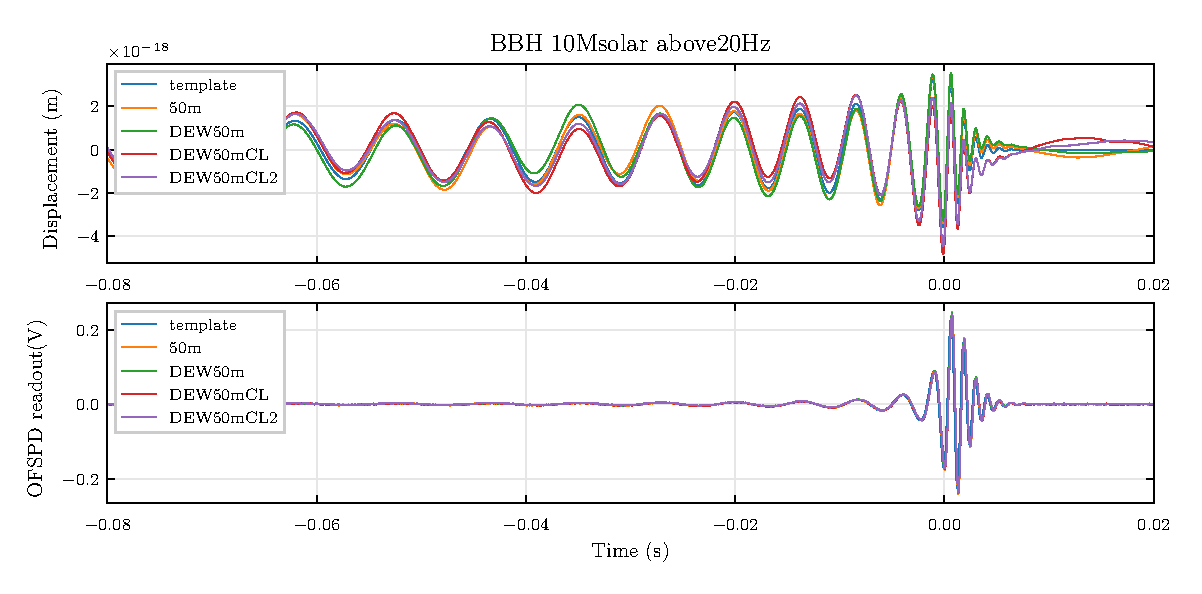
\includegraphics[width=0.93\textwidth]{figure/inj/10.eps}
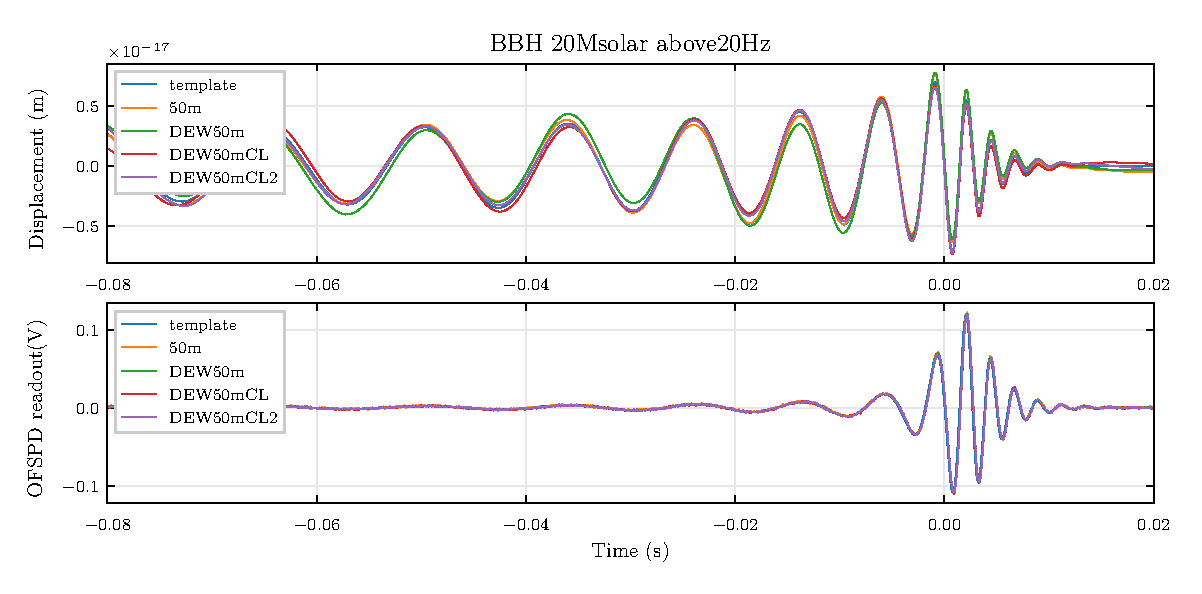
\includegraphics[width=0.93\textwidth]{figure/inj/20.eps}
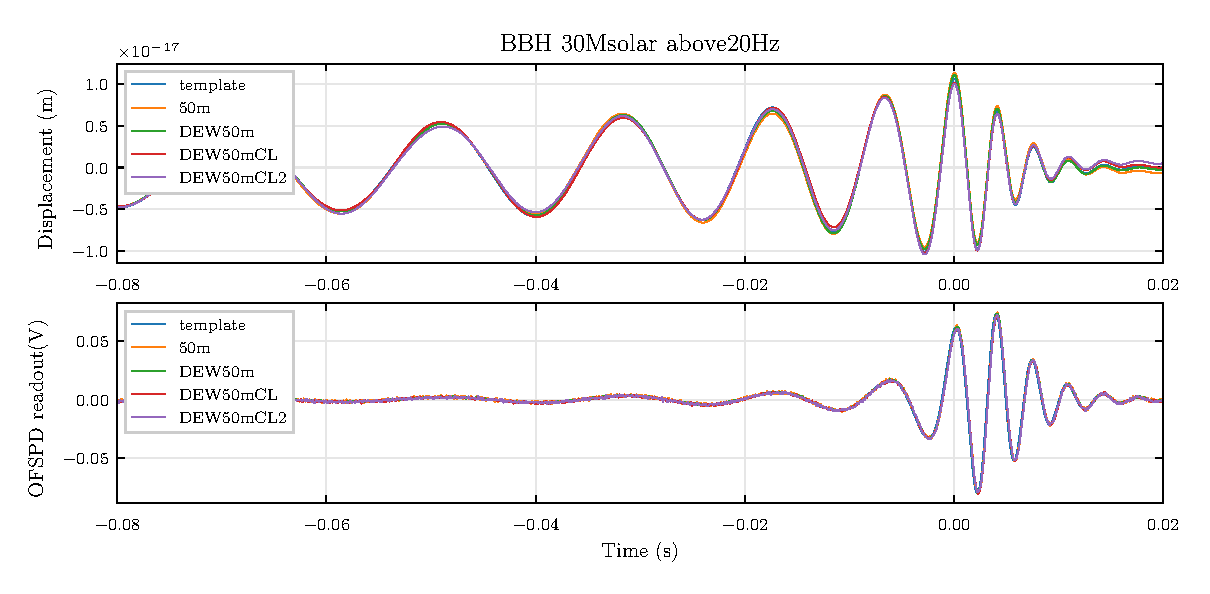
\includegraphics[width=0.93\textwidth]{figure/inj/30.eps}
\caption[Injected Binary Blackhole Merger Signals]{Injected Binary Blackhole Merger Signals. The lower panel of each plots is the electrical readout from a photodiode (OFSPD) in the PCal. It is proportional to the intensity of the PCal laser beam. The upper panel of each plots shows the theoretically estimated ETM displacement by applying $1/\omega^2$ force-to-length transfer function to the observed laser intensity. The meaning of the legend is explained in Table~\ref{tab:injlegend}}
\label{fig:bbhinj}
\index{figures}
\end{figure}


\begin{table}[hbt!]
\centering
\begin{tabular}{ll}
\hline
Label in legend  & Description        \\
\hline
template    & The data in the injected signal file.\\
50m         & Without PCal, only through 50m+50m cables as a test of Digital System.\\
DEW50m      & Same as the 50m but includes De-Whitening Filter and its digital inverse.   \\
DEW50mCL    & With De-Whitening filter, its digital inverse, and PCal.   \\
DEW50mCL2   & Same as DEW50mCL, a second time test with the identical setup.    \\
\hline
\end{tabular}
\caption{Explanation of legends in the injection result}
\label{tab:injlegend}
\index{tables}
\end{table}



